% -*- root: ../main.tex -*-
% Chapter Template

\chapter{Background} % Main chapter title

\label{ChapterBackground} % Change X to a consecutive number; for referencing this chapter elsewhere, use \ref{ChapterX}

\lhead{\chaptername~\thechapter. \emph{Background}} % Change X to a consecutive number; this is for the header on each page - perhaps a shortened title
\begin{quote}
This chapter provides the background knowledge that is required to understand this research and why it was undertaken. Insight is given into the applications of lightning current models, including induced currents on transmission lines and lightning frequency component analyses. The terminology used in the IEC lightning protection standard is defined giving insight into the reason for approximating the Heidler function. The Heidler function and the double exponential function are also defined and discussed. A literature review is carried out showing some of the work done by other researchers in obtaining approximations to the Heidler function.
\end{quote}

%----------------------------------------------------------------------------------------
%    Overview
%----------------------------------------------------------------------------------------

\section{Overview}
\label{sec:background_overview}
In order to understand the research presented in this dissertation, there are certain concepts that require further description. In the previous chapter the research questions of what, why and how are answered. However, very little detail is given about the concepts and ideas mentioned. This chapter explains a few of the applications where it is appropriate to utilise lightning current models. Key components of the IEC~62305-1 (part one of the lightning protection standard) are explained. Two of the more common lightning current models are detailed and some of the approximations that have been developed by other researchers are detailed. This all gives some background relating to the study.

%----------------------------------------------------------------------------------------
%    Application for Lightning Current Models
%----------------------------------------------------------------------------------------

\section{Application for Lightning Current Models}
\label{sec:background_applications}
There are several instances when there is a requirement to use a lightning current model such as in the design of \glspl{lps}. Two of the more specific cases where lightning current models are used are detailed below. These include current path analyses using return stroke modelling and the need for the frequency components of lightning.
%-----------------------------------
%    Current Path Analyses
%-----------------------------------
\subsection{Current Path Analyses}
\label{sub:background_lemp}
Return stroke models are characterised into four primary classes, namely gas dynamics model, electromagnetic model, distributed circuit model and the engineering model \cite{Paolone2009,Rakov2003,Rakov2009}. The engineering model is the primary model used when looking at induced effects on power lines.

\begin{figure}[htbp]
    \centering
    \subfigure[]{
        \tikzsetnextfilename{PhysicalModel}
        %!tikz editor 1.0
%!tikz source begin
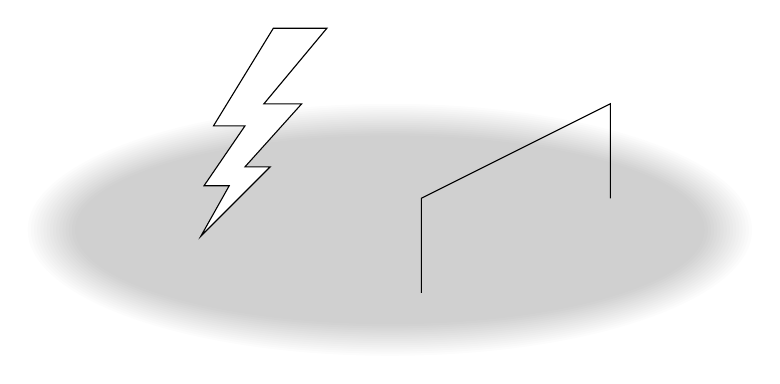
\begin{tikzpicture}[scale=0.8, transform shape]
%\fill [black, fill opacity = 0.075] (2,0.8) ellipse [x radius = 5, y radius = 1.5];

\foreach \i in {0,2,...,30}
        \fill [black, fill opacity = 1/100] (2,0.8)
          ellipse [x radius = 5+\i/40, y radius = 1.5+\i/60];

\fill [draw,fill=white] (1,4) to ++ (-1,-1.2) to ++ (0.6,0) to ++ (-0.9,-1) to ++ (0.4,0) to ++ (-1.1, -1.1) node (bot) {} to ++ (0.45,0.8) to ++ (-0.4,0) to ++ (0.65,0.95) to ++ (-0.5,0) to ++ (0.95,1.55) -- cycle;

\draw (bot) ++ (3.5,-0.9) to ++ (0,1.5) to ++(3,1.5) to ++ (0,-1.5);
\end{tikzpicture}
%!tikz source end

        \label{fig:physical_model}
    }
    \subfigure[]{
        \tikzsetnextfilename{TransmissionLineModel}
        %!tikz editor 1.0
%!tikz source begin
\begin{tikzpicture}[american currents, scale=0.8, transform shape]
\foreach \i in {0,2,...,30}
        \fill [black, fill opacity = 1/100] (2,0.8)
          ellipse [x radius = 5+\i/40, y radius = 1.5+\i/60];

\fill [fill=none] (1,4) to ++ (-1,-1.2) to ++ (0.6,0) to ++ (-0.9,-1) to ++ (0.4,0) to ++ (-1.1, -1.1) node (bot) {} to ++ (0.45,0.8) to ++ (-0.4,0) to ++ (0.65,0.95) to ++ (-0.5,0) to ++ (0.95,1.55) -- cycle;

\draw (bot) node[rground] {} to [I=$i(t)$] ++ (0,0.8) to ++(0,2.7);

\draw (bot) ++ (3.5,-0.4) node[rground]{} to[generic=$Z_0$] +(0,2);
\draw (bot) ++ (6.5,2.6) to[transmission line, *-*]++(-3,-1);
\draw (bot) ++ (6.5,2.6) to[generic=$Z_0$] ++ (0,-2) node[rground]{};

\end{tikzpicture}
%!tikz source end

        \label{fig:tr_line_model}
    }
    \caption{\subref{fig:physical_model} Physical and \subref{fig:tr_line_model} Transmission Line models of a lightning strike close to a transmission line that induces over-voltages on the line.}
    \label{fig:induced_voltage_models}
\end{figure}
\figref{fig:induced_voltage_models} shows the \subref{fig:physical_model} physical and \subref{fig:tr_line_model} return stroke models for a lightning strike in close proximity to a transmission line. From these figures it can be seen that when modelling a lightning strike occurring in close proximity to a transmission line, the lightning channel is modelled as a monopole with a perfectly conductive ground and a vertical current path \cite{Paolone2009,Baba2007,McAfee2015}.

Information about the \gls{em} fields are required when calculating the induced effects of the lightning strike on the transmission line. The induced currents can be calculated by integrating the different components of the \gls{em} fields as outlined by \citeauthor{Agrawal1980} \cite{Agrawal1980}. The \gls{lemp} equations need to be determined before calculating the \gls{em} fields. The equations for the \gls{em} fields can be seen in \eqnrefs{eqn:e_field}{eqn:b_field} respectively. These are defined by \citeauthor{Uman1975} as the \gls{lemp} equations \cite{Uman1975}.
\begin{dmath}
    E_z \left( D,t \right)=\frac{1}{2\pi\epsilon_0}\left[\int_{0}^{H}\frac{2 - 3\sin^{2}{\theta}}{R^3} \times \int_{0}^{t} i \left( z, \tau - \frac{R}{c} \right) \, d\tau dz \\ + \int_{0}^{H} \frac{2 - 3\sin^{2}{\theta}}{c R^2} i \left( z, t - \frac{R}{c} \right) \, dz - \int_{0}^{H} \frac{\sin^{2}{\theta}}{c^2 R} \frac{\partial i\left ( z, t - \frac{R}{c} \right )}{\partial t} \, dz \right ]
    \label{eqn:e_field}
\end{dmath}
\begin{dmath}
    B_{\phi} \left( D,t \right) = \frac{\mu_0}{2\pi} \int_{0}^{H} \frac{\sin{\theta}}{R^2} i \left ( z, t - \frac{r}{c} \right ) \, dz + \frac{\mu_0}{2\pi} \int_{0}^{H} \frac{\sin{\theta}}{cR} \frac{\partial i \left ( z, t - \frac{R}{c} \right )}{\partial t} \, dz
    \label{eqn:b_field}
\end{dmath}
The full extent of what these equations mean is beyond the scope of this study. However, what is clear is that these equations utilise the return stroke model, $i \left( z, t \right)$. This expression for the lightning current along a path can be defined by different models as in \cite{Paolone2009,ZhangFeizhouandLiuShanghe2002,Nucci2003}. All the models hold the form shown in \eqnref{eqn:rsm} where $u(t)$ is the Heaviside function, $P(z')$ is the height-dependent current attenuation factor and $i(0,t)$ is the lightning channel base current which as the name suggests is the current as measured from the base of the object that is struck \cite{Paolone2009,ZhangFeizhouandLiuShanghe2002,Javor2011}.
\begin{equation}
    i(z',t)=u\left( t - \frac{z'}{v}\right) P \left( z' \right) i \left( 0,t - \frac{z'}{v} \right)
    \label{eqn:rsm}
\end{equation}
In short, there are two steps of integration required to calculate induced currents on transmission lines \cite{Nucci2010,Nucci2003,Paolone2009}.
\begin{enumerate}
    \item Integrate some model of the lightning channel base current to obtain the \gls{em} fields.
    \item Integrate the \gls{em} fields using the equations defined by \citeauthor{Agrawal1980} to obtain the induced currents.
\end{enumerate}

%Therefore, by choosing an appropriate lightning channel base current, the induced effects on nearby transmission lines can be calculated.
Referring back to \figref{fig:induced_voltage_models}, the induced effects on a nearby transmission line can be calculated by modelling the lightning event as in \figref{fig:tr_line_model} and choosing an appropriate lightning channel base current. Clearly from the equations above, at least the second integral of this channel base current is required. Using an accurate lightning channel base current leads to very complex models that require long computer simulations because of numerical integration \cite{Paolone2009}. \secref{sec:background_current_waveshape_models} details two of the more common equations used as lightning channel base current models.

%-----------------------------------
%    Frequency Components of Lightning Currents
%-----------------------------------
\subsection{Frequency Components of Lightning Currents}
\label{sub:background_frequency_components_of_lightning_currents}
Obtaining frequency components of a lightning strike are important for studies such as that done by \citeauthor{Lee2014}, where they are studying the effects of the lightning frequency components on human injury caused by a lightning strike \cite{Lee2014}. In this study, \citeauthor{Lee2014} utilise the double exponential function to obtain the frequency components of a lightning strike. The frequency components in the double exponential are found to be an order of magnitude different to those recommended by the standards \cite{1422588}.

The reason for such a study is that the sharp rise in the lightning current creates a broadband current. Without using the Heidler function for such applications, it is difficult to standardise testing across the different fields of interest.

%----------------------------------------------------------------------------------------
%    IEC~62305 - Lightning Protection Standard
%----------------------------------------------------------------------------------------

\section{IEC~62305-1 - Lightning Protection Standard}
\label{sec:background_iec62305}
The IEC~62305 is the lightning protection standard containing four parts. Where part one focuses on the general principles of lightning protection and parts two to four focus on more specific areas of lightning protection. IEC~62305-1 details all the relevant components of a lightning flash as well as all the terminology and standard values to utilise when designing systems such as \glspl{lps}.

\figref{fig:IECWave} shows an adaptation of Figure A.1 from the standard. This figure shows how the different stroke currents, such as the 0.25/100 and 10/350 are composed. $T_1$ is the rise time (number before the `/') and $T_2$ is the fall time (number after the `/').
\inputtikzfig{IECWave}{IECWave}{Definitions of short stroke parameters adapted from \cite{IEC623051}}

Figures A.3 and A.4 in the standard show typical waveshapes expected from both downward and upward lightning flashes respectively. The three components identified in these images are the first short stroke, the subsequent short stroke and the long stroke. The first and subsequent short strokes are seen to be high current impulses with a sharp rise and a slower decay. The long stroke on the other hand is a lower current that is maintained for a comparatively long time.

Table A.1 in the standard shows the values that should be used in system designs. The values given here are the maximum change in current, the charge, the peak current, etc. With these values, systems can be designed to different \glspl{lpl}. The values given in this table are based on the original studies done by \citeauthor{Anderson1980} and \citeauthor{Berger1975} on lightning currents \cite{Anderson1980,Berger1975}. The standard typically makes use of the upper end values to protect against more lightning events. For example, a system with a higher current rating will be protected against a lower current lightning strike.

In order to simulate lightning currents in \gls{lps} design, the standard identifies a function that creates a waveshape with the characteristics outlined in Table A.1 of the standard. This function is the Heidler function with a specific configuration ($n = 10$) (see \secref{sub:background_heidler}). This function can be used to create any lightning current waveshape with the two of interest in the standard being the 10/350 (first short stroke) and the 0.25/100 (subsequent short stroke). These two waveshapes are simulated using the parameters specified in Table B.1 in the standard for the different \glspl{lpl} and stroke types \cite{IEC623051}.

%----------------------------------------------------------------------------------------
%    Current Waveshape Models
%----------------------------------------------------------------------------------------

\section{Current Waveshape Models}
\label{sec:background_current_waveshape_models}
The IEC lightning protection standard details the Heidler function with a specific configuration as the standardised waveshape for lightning current simulations. There are several lightning current models defined in the literature with the two most popular being the Heidler and the double exponential. There are also applications that use a combination of the two \cite{Javor2011,Nucci2003,Pavanello2007}. This section gives some background into these two equations and their properties.

%-----------------------------------
%    The Double Exponential Model
%-----------------------------------
\subsection{The Double Exponential Model}
\label{sub:background_double_exponential}
The double exponential function is defined in \eqnref{eqn:dexp}.
\begin{equation}
    i_e \left( t \right) = \frac{I_o}{A}\left( e^{-\alpha t} - e^{-\beta t} \right)
    \label{eqn:dexp}
\end{equation}
Where: \\
\begin{tabular}{cll}
    $I_0$ & = & Peak current [A] \\
    $A$ & = & Peak current correction \\
    $\alpha$ & = & Decay time constant [1/s] \\
    $\beta$ & = & Rise time constant [1/s]
\end{tabular}\\\\
The double exponential model is often used in place of the Heidler function because it can be integrated. However the waveshape produced by the double exponential equation is not physically realistic because the maximum current steepness occurs at time $t=0$ \cite{ZhangFeizhouandLiuShanghe2002,Lovric2013,Heidler2002,Delfino2012}. Moreover, this function does not allow for waveshapes that comply with Table A.1 in the IEC~62305-1 standard. For instance, a subsequent short stroke for \gls{lpl}-I would have a maximum current steepness of about 545 kA/\usec, which is far greater than the maximum value outlined in the standard of less than 200 kA/\usec \cite{Heidler2008}. Another disadvantage to using this equation is that it is not easily adjustable, the parameters are not easily obtained for different waveshapes \cite{Javor2011}.

%-----------------------------------
%    The Heidler Function
%-----------------------------------
\subsection{The Heidler Function}
\label{sub:background_heidler}
To avoid the disadvantages of the double exponential equation, the Heidler function is used. This can be seen in \eqnref{eqn:HF}.
\begin{equation}
i_h \left( t \right) = \frac{I_0}{\eta} \frac{{\left (\frac{t}{\tau_1} \right )}^{n_h}}{1 + {\left (\frac{t}{\tau_1} \right )}^{n_h}} e^{-\frac{t}{\tau_2}}
\label{eqn:HF}
\end{equation}

Where: \\
\begin{tabular}{cll}
    $I_0$ & = & Peak current [A] \\
    $\eta$ & = & Peak current correction \\
    $\tau_1$ & = & Rise time constant [s] \\
    $\tau_2$ & = & Decay time constant [s] \\
    $n_h$ & = & Heidler steepness factor
\end{tabular}\\\\
This equation more realistically approximates a lightning return stroke and the peak current correction can be calculated using \eqnref{eqn:eta} \cite{ZhangFeizhouandLiuShanghe2002,Lovric2013,Delfino2012,Javor2011,Heidler1999}.
\begin{equation}
    \eta =e^{-\frac{\tau _1}{\tau _2} \left(\frac{n_h \tau _2}{\tau _1}\right)^{\frac{1}{n_h}}}
    \label{eqn:eta}
\end{equation}
\eqnref{eqn:dHF} shows the first derivative of the Heidler function.
\begin{equation}
    i'_h \left( t \right) = \frac{I_0}{\eta} \left( \frac{n_h t^{n_h - 1} \tau_1^{n_h}}{\left(\tau_1^{n_h} + t^{n_h} \right)^2} - \frac{t^{n_h}}{\tau_2 \left(\tau_1^{n_h} + t^{n_h} \right)} \right) e^{-\frac{t}{\tau_2}}
    \label{eqn:dHF}
\end{equation}

The IEC~62305-1 standard makes use of a specialised form of the Heidler function where $n_h = 10$. Using this form of the equation, there are values for the other parameters in the standard that can be used to simulate both first and subsequent short strokes \cite{IEC623051,Heidler2008}.

The disadvantage of the Heidler function is that there is no analytical integral and hence no analytical expression for the Heidler function in the frequency domain \cite{ZhangFeizhouandLiuShanghe2002,Lovric2013}. This creates problems when performing analyses such as those mentioned in \secref{sec:background_applications} above.

%----------------------------------------------------------------------------------------
%    Heidler Function Approximations
%----------------------------------------------------------------------------------------

\section{Heidler Function Approximations}
\label{sec:background_approximations}
As there are is no analytical integral to the Heidler function, there are many researchers working towards an approximation that can be used in its place for applications such as those mentioned in \secref{sec:background_applications}. This section discusses a few of these approximations with the disadvantages associated with each one.

\citeauthor{ZhangFeizhouandLiuShanghe2002} developed a function that they call the \textit{Pulse function} \cite{ZhangFeizhouandLiuShanghe2002}. According to their study, this function produces a maximum error of 0.5\% with the waveshapes they used. However, this function is a modified form of the double exponential function and it requires very complex methods to determine the parameters used in the equation.

\citeauthor{Heidler2002} approximate the Heidler function utilised in the IEC~62305-1 standard \cite{Heidler2002}. This approximation has an analytical integral but the equation is specific to the subsequent short stroke. There is no general form of this approximation and so this equation cannot be easily manipulated. Their study also details several other approximations to the Heidler function but all with other applications. They all have the disadvantage that they cannot be integrated analytically.

\citeauthor{Delfino2012} conduct a study in which they develop a Prony series approximation to the Heidler function \cite{Delfino2012}. The mathematics required for this approximation is very complex limiting its use in engineering applications. Each scenario is different as there is no truly generalised form and the number of terms used affects the error associated with the approximation. This would be difficult to use for engineering applications.

\citeauthor{Javor2011} develop a new approximation that they call the \textit{\gls{ncbc}} \cite{Javor2011,Javor2012}. This function contains some complicated mathematics and it is a piecewise function which implies that there are discontinuities when taking the analytical derivative with step functions. The approximation also contains incomplete gamma functions which are defined as integrals and hence further complicate the mathematics \cite{Gautschi:1979:CPI}. There is no analytical Fourier transform to this approximation \cite{Javor}.

\citeauthor{Vujevic2009} define their version of the \textit{exponential approximation} that is fixed for $n_h=10$ \cite{Vujevic2009,Vujevic2010a}. The mathematics presented in their study is extremely complicated and they introduce several new unknown parameters. The approximation is not as intuitive as the Heidler function. The frequency response presented is not as expected at higher frequencies; it does not roll off as it does in the standard.

All of the approximations above have one or more disadvantage or limitation. Overall the problems are that the mathematics are very complicated and it would be very difficult to simply substitute these equations in place of the Heidler function in the IEC~62305-1. The approximation in this dissertation provides an approximation, with an analytical integral, for use in engineering applications that does not have these limitations.

%----------------------------------------------------------------------------------------
%    Conclusion
%----------------------------------------------------------------------------------------

\section{Conclusion}
\label{sec:background_conclusion}
This chapter has given the background information relevant to this study. This includes all the terminology, equations, applications and a literature review.

The following chapter details the approximation that is developed in this study. The development of the function is detailed and all its properties are discussed in isolation.
